\documentclass{beamer}

\usepackage{imperial-beamer-style}
\usepackage[backend=bibtex,citestyle=numeric-comp,sorting=nty,style=authortitle]{biblatex}
\addbibresource{main.bib}
%\usetheme{Warsaw}

\title{ISO Presentation}
\subtitle{Quantum Programming}
\date{6 May 2020}
\author[Tristan \textsc{Nemoz}]{Tristan \textsc{Nemoz}\\{\small Supervisor: Mario \textsc{Berta}}}

\usepackage{amsmath}

\DeclareMathOperator{\polylog}{polylog}
\DeclareMathOperator{\poly}{poly}
\DeclareMathOperator{\sgn}{sgn}

\usepackage{caption}
\usepackage{subcaption}
\usepackage{tikz}
\usetikzlibrary{arrows, shapes.gates.logic.US, calc, quantikz}
\usepackage{forest}
\usepackage{blochsphere}
\usepackage{tikz-3dplot}
\usetikzlibrary{3d}

\tikzset{
    invisible/.style={opacity=0,text opacity=0},
    visible on/.style={alt=#1{}{invisible}},
    alt/.code args={<#1>#2#3}{%
      \alt<#1>{\pgfkeysalso{#2}}{\pgfkeysalso{#3}} % \pgfkeysalso doesn't change the path
    },
}
\forestset{
  visible on/.style={
    for tree={
      /tikz/visible on={#1},
      edge+={/tikz/visible on={#1}}}}}

\begin{document}

\begin{frame}
\maketitle
\end{frame}

\section{Introduction}

\begin{frame}{Quantum Computing applied to Machine Learning}
    \begin{itemize}
        \item Goal: exponential speed-up\pause
        \item HHL\only<2->{\footcite{HHL}} (2009): $O(n)\to O\left(\log(n)\,\kappa^2\right)$\pause
        \item \textcolor<4->{red}{Quantum Recommendation Systems}\only<3->{\footcite{QRS}} (2016): $O\left(n^2\right)\to O(\poly(k)\,\polylog(m\,n))$
    \end{itemize}
\end{frame}

\section{Problem statement}

\begin{frame}{Real-world problem overview}
    \begin{itemize}
        \item $m$ users can rate $n$ products\pause\ (binary voting)\pause
        \item Not all ratings are known\pause
        \item Can we predict whether user $j$ will like product $k$?
    \end{itemize}
\end{frame}

\begin{frame}{Mathematical description}
    \begin{block}{Binary recommendation system}
        Let $\mathbf{P}\in\{0\,;\,1\}^{m\times n}$, whose coefficients are known with a given probability. A quantum recommendation system, given $\hat{\mathbf{P}}$ the incomplete respresentation of $\mathbf{P}$ and an user $j$, predicts $k$ such that $\mathbf{P}_{j,k}=1$ with high probability.
    \end{block}\pause
    Impossible problem without assumptions
\end{frame}

\begin{frame}{Problem assumptions}
    \begin{exampleblock}{The low-rank assumption}
        Let $\mathbf{P}$ be the unknown preference matrix. For a given precision parameter $\varepsilon$, there exists a rank-$k$ matrix $\mathbf{T}$ such that:
        
        \[\|\mathbf{P}-\mathbf{T}\|_F\leqslant\varepsilon\,\|\mathbf{P}\|_F\,.\]
    \end{exampleblock}\pause
    $\implies$ there are $k$ types of \textcolor<3>{red}{typical} users.\pause\pause
    
    \begin{exampleblock}{Problem initialization}
        $\mathbf{P}$ can be sampled into $\hat{\mathbf{P}}$ such that $\hat{\mathbf{P}}$ holds the low-rank assumption. Hence, $\varepsilon$ is assumed to be known.
    \end{exampleblock}
\end{frame}

\begin{frame}{A Quantum Recommendation System}
    \begin{itemize}
        \item Introduced in 2016\footcite{QRS}\pause
        \item Offers an exponential speed-up regarding to classical algorithms at that time\pause
        \item \textcolor<4>{red}{No practical implementation proposed}\pause\pause
    \end{itemize}
    
    \begin{block}{Problem statement}
        How does the real-world implementation of the Quantum Recommendation System algorithm differs from its theoretic implementation?
    \end{block}
\end{frame}

\section{Quantum Computing}
\subsection{Classical computing parallel}

\begin{frame}{Classical computing}
    \begin{itemize}
        \item Operates on bit-strings 0110110001\pause
        \item Bits are elements of \(\{0\,;\,1\}\)\pause
        \item Some operations are reversible, \textcolor<9->{red}{some are not}\pause
        \item Cloning or setting a bit to 0 can be done in $O(1)$\pause
        \item Operates with a limited set of gates:\pause
        
        \begin{figure}[ht]
            \centering
            \begin{subfigure}[b]{.3\textwidth}
                \centering
                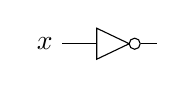
\begin{tikzpicture}
                    \node[draw=none] (x) at (0, 1) {$x$};
                    \node[not gate US, draw] at ($(x) + (0.8, 0)$) (notx) {};
                    \draw (x) -- (notx.input);
                    \draw (notx.output) -- ([xshift=0.2cm]notx.output);
                \end{tikzpicture}
                \caption{NOT gate}
            \end{subfigure}\pause
            \begin{subfigure}[b]{.3\textwidth}
                \centering
                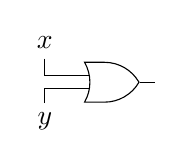
\begin{tikzpicture}
                    \node (x) at (0, 1) {$x$};
                    \node (y) at (0, 0) {$y$};
                    \node[or gate US, draw, rotate=0, logic gate inputs=nn] at ($(0.8, 0.5)$) (xory) {};
                    \draw (x) |- (xory.input 1);
                    \draw (y) |- (xory.input 2);
                    \draw (xory.output) -- ([xshift=0.2cm]xory.output);
                \end{tikzpicture}
                \caption{\textcolor<9->{red}{OR gate}}
            \end{subfigure}\pause
            \begin{subfigure}[b]{.3\textwidth}
                \centering
                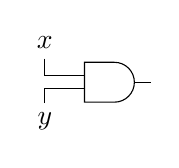
\begin{tikzpicture}
                    \node (x) at (0, 1) {$x$};
                    \node (y) at (0, 0) {$y$};
                    \node[and gate US, draw, rotate=0, logic gate inputs=nn] at ($(0.8, 0.5)$) (xory) {};
                    \draw (x) |- (xory.input 1);
                    \draw (y) |- (xory.input 2);
                    \draw (xory.output) -- ([xshift=0.2cm]xory.output);
                \end{tikzpicture}
                \caption{\textcolor<9->{red}{AND gate}}
            \end{subfigure}
            \caption{Classical gates}
        \end{figure}
    \end{itemize}
\end{frame}

\begin{frame}{Quantum computing}
    \begin{itemize}
        \item Operates on \textbf{qubits}-strings $\ket{q_1}\,\ket{q_2}\,\ket{q_3}\,\ket{q_4}\,\ket{q_5}$\pause
        \item Qubits are \textbf{normalized vectors of} $\mathbf{C}^2$\pause
        \item \textbf{All} operations\only<4->{ (aside from measuring)} are reversible\pause\pause
        \item Cloning or setting a qubit to $\ket{0}$ is \textbf{impossible} \only<6->{(in the general case)}\pause\pause
        \item Operates with a limited set of matrices/gates:\pause
        
        \begin{figure}[ht]
            \centering
            \begin{subfigure}[b]{.3\textwidth}
                \centering
                \begin{quantikz}
                    \qw & \gate{\mathbf{R}_z(\theta)} & \qw
                \end{quantikz}
                \caption{The $\mathbf{R}_z(\theta)$ gate}
            \end{subfigure}\pause
            \begin{subfigure}[b]{.3\textwidth}
                \centering
                \begin{quantikz}
                    \qw & \ctrl{1} & \qw\\
                    \qw & \gate{\mathbf{Z}} & \qw
                \end{quantikz}
                \caption{The $\mathsf{C}-\mathbf{Z}$ gate}
            \end{subfigure}\pause
            \begin{subfigure}[b]{.3\textwidth}
                \centering
                \begin{quantikz}
                    \qw & \gate{\mathbf{R}_{xy}(\theta,\varphi)} & \qw
                \end{quantikz}
                \caption{The $\mathbf{R}_{xy}(\theta,\varphi)$ gate}
            \end{subfigure}
            \caption{Quantum gates}
        \end{figure}
    \end{itemize}
\end{frame}

\subsection{Quantum Computing formalism}

\begin{frame}{Quantum Computing formalism}
    \begin{block}{Qubits}
        A qubit \ket{q} is a normalized vector of $\mathbf{C}^2$. We denote:
        
        \[\ket{q}=\begin{pmatrix}\alpha\\\beta\end{pmatrix}\pause=\alpha\,\begin{pmatrix}1\\0\end{pmatrix} + \beta\,\begin{pmatrix}0\\1\end{pmatrix}\pause=\alpha\,\ket{0}+\beta\,\ket{1}.\]
        
        \pause A qubits-string is called a \textbf{quantum register}.\pause\ It is mathematically described as the tensor product of these qubits, that is:
        
        \[\ket{q_1}\,\ket{q_2}\,\cdots\,\ket{q_n}=\bigotimes_{j=1}^n\ket{q_k}\,.\]
    \end{block}
\end{frame}

\begin{frame}{The Bloch sphere}
    A qubit \ket{q} can be represented on the so-called Bloch sphere:\pause
    
    \begin{figure}[ht]
        \centering
        \begin{subfigure}[b]{.47\textwidth}
            \centering
            \begin{blochsphere}[ball=3d,opacity=0.1, radius=1.5cm, axisarrow=->]
                \drawBallGrid[style={opacity=1,ultra thin}]{30}{30}
                \drawAxis[scale=1.2]{0}{0}
                \drawAxis[scale=1.8]{90}{90}
                \drawAxis[scale=1.4]{90}{0}
                \labelLatLon{z}{90}{0};
                \labelLatLon{y}{0}{0};
                \labelLatLon{x}{0}{90};
                \labelLatLon{1}{-90}{90};
                \node[above,{shift=(0,0.4,0)}] at (z) {$z$};
                \node[above,{shift=(0.8,0,0)}] at (y) {$y$};
                \node[above,{shift=(0,0,1.8)}] at (x) {$x$};
                \node[below,{shift=(0,-0.4,0)}] at (1) {\phantom{\ket{1}}};
            \end{blochsphere}
        \end{subfigure}\pause
        \begin{subfigure}[b]{.47\textwidth}
            \centering
            \begin{blochsphere}[ball=3d,opacity=0.1, radius=1.5cm, statecolor=red, statewidth=1.2pt, axisarrow=->]
                \drawBallGrid[style={opacity=1,ultra thin}]{30}{30}
                \drawAxis[scale=1.2]{0}{0}
                \drawAxis[scale=1.8]{90}{90}
                \drawAxis[scale=1.4]{90}{0}
                \labelLatLon{0}{90}{0};
                \labelLatLon{1}{-90}{90};
                \labelLatLon{y}{0}{0};
                \labelLatLon{x}{0}{90};
                \node[above,{shift=(0,0.4,0)}] at (0) {\ket{0}};
                \node[below,{shift=(0,-0.4,0)}] at (1) {\ket{1}};
                \node[above,{shift=(0.8,0,0)}] at (y) {$\frac{\ket{0}+\mathrm{i}\,\ket{1}}{\sqrt{2}}$};
                \node[above,{shift=(0,0,2.4)}] at (x) {$\frac{\ket{0}+\ket{1}}{\sqrt{2}}$};\pause
                \drawStatePolar{state}{45}{-30}
            \end{blochsphere}
        \end{subfigure}
        \caption{The Bloch Sphere}
    \end{figure}
\end{frame}


\begin{frame}{Quantum Computing principles}
    \begin{itemize}
        \item Possibility to encode information with qubits-strings\pause
        \item Linearity allows to apply operations on several qubits-string at a time\pause
        \item Possibility to get a probabilistic view of a qubit at the price of forcing it into a certain state.\pause\ \textcolor{red}{Measurement destroys information.} 
    \end{itemize}
\end{frame}

\section{Implementing a Quantum Recommendation system}

\begin{frame}{Implementing a Quantum Recommendation system}
    \begin{itemize}
        \item The real-world implementation of the algorithm is quite straight-forward, except for:\pause
        \begin{itemize}
            \item \textcolor<5->{red}{Loading a vector stored in a classical structure as a quantum state}\pause
            \item Applying the Quantum Phase Estimation subroutine\pause
            \item Comparing a qubits-string and a bits-string
        \end{itemize}
    \end{itemize}
\end{frame}

\begin{frame}{Loading a vector as a quantum state}
    \begin{block}{Loading a vector as a quantum state}
        Let \(\mathbf{x}\in\mathbf{R}^n\) be a normalized vector.\pause Then, its associated quantum state is:
        
        \[\ket{x}=\sum_{j\in\{0\,;\,1\}^{\left\lceil\log_2(n)\right\rceil}}\mathbf{x}_j\,\ket{q}\,.\]\pause
        
        Loading $\mathbf{x}$ means creating \ket{x} from $\ket{0}^{\otimes\left\lceil\log_2(n)\right\rceil}$ with a polylogarithmic number of gates\footnotemark.
    \end{block}\only<3->{\footcitetext{Prakash}}
\end{frame}

\begin{frame}{Quantum RAM}
    \begin{block}{QRAM\footnotemark}
        A QRAM is a binary tree whose leaves stores the coefficients of a vector $\mathbf{x}$ and whose nodes stores the sum of its leaves values.\pause
        
        \begin{figure}[ht]
            \centering
            \scalebox{0.825}{
                \begin{forest}
                    [$1$, visible on=<2->, for children={visible on=<3->}
                        [$\mathbf{x}_1^2+\mathbf{x}_2^2$, for children={visible on=<4->}
                            [$\mathbf{x}_1^2{,}\sgn\left(\mathbf{x}_1\right)$]
                            [$\mathbf{x}_2^2{,}\sgn\left(\mathbf{x}_2\right)$]
                        ]
                        [$\mathbf{x}_3^2+\mathbf{x}_4^2$, for children={visible on=<4->}
                            [$\mathbf{x}_2^3{,}\sgn\left(\mathbf{x}_3\right)$]
                            [$\mathbf{x}_2^4{,}\sgn\left(\mathbf{x}_4\right)$]
                        ]
                    ]
                \end{forest}
                }
            \caption{An example of a QRAM tree}
        \end{figure}

    \end{block}\footcitetext{Prakash}
\end{frame}

\begin{frame}{Loading from QRAM}
    \begin{itemize}
        \item Method described in \cite{QLSPrimer}\pause
        \item Uses $2^k$ rotations gates around the $y$-axis at level $k$ of the tree whose angle are determined using QRAM\pause
        \item Goal: parallelize the execution of the rotations using superposition
    \end{itemize}
\end{frame}

\begin{frame}{Parallel execution}
    \begin{block}{Parallel execution of controlled rotations}
        Let \ket{x} be a $n$-qubits quantum register and \ket{0} be a target qubit.\pause\ Parallel execution of controlled rotations consists in applying on the target qubit a rotation around the $y$-axis of angle $\theta_k$ only if the first quantum register is in state \ket{k}\pause\ in time constant with respect to $n$.
    \end{block}
    
    \pause
    
    \begin{exampleblock}{QRAM function assumption}
        It is possible, using QRAM, to design a gate $\mathbf{L}_k$ such that:
        
        \[\mathbf{L}_k\,\ket{k}\,\ket{0}^{\otimes t} = \ket{k}\,\ket{\overline{\theta_k}}\]
        
        where $\overline{\theta_k}$ is the best $t$-bits approximation of $\theta_k$.
    \end{exampleblock}
\end{frame}

\begin{frame}{A simpler problem}
    \begin{block}{Parallel execution of rotations}
        It is possible to get the state $\ket{\theta}\,\mathrm{e}^{\mathrm{i}\,\theta}\,\ket{x}$ from the state $\ket{\theta}\,(\alpha\,\ket{0}+\beta\,\ket{1})$\pause\ in time $O(1)$.
    \end{block}\pause
    
    \begin{exampleblock}{The $z$-rotation}
        Given an angle $\theta$, the rotation around the $z$-axis of the Bloch sphere is given by the gate:
        
        \[\mathbf{R}_z(\theta)=\begin{pmatrix}1&0\\0&\mathrm{e}^{\mathrm{i}\,\theta}\end{pmatrix}\,.\]
    \end{exampleblock}
\end{frame}

\begin{frame}{Parallel execution of rotations}
    Let $\theta_i\in\{0\,;\,1\}$.\pause
    
     \begin{figure}[ht]
        \centering
        \begin{quantikz}
            \lstick{\ket{\theta_i}} & \gate{\mathbf{R}_z\left(\frac{1}{2^k}\right)} & \qw\rstick{\ket{\psi}}
        \end{quantikz}
        \caption{Effect of the $z$-rotation on a qubit}
     \end{figure}
     
     \pause
     
     \[\ket{\psi}=\pause\begin{cases}\ket{0}&\text{if } \theta_i=0\pause\\\mathrm{e}^{\mathrm{i}\,2^{-k}}\,\ket{1}&\text{if }\theta_i=1\end{cases}\pause=\mathrm{e}^{\mathrm{i}\,\textcolor<7->{red}{\theta_i}\,2^{-k}}\,\ket{\theta_i}\]
\end{frame}

\begin{frame}{Parallel execution of rotations}
    Let $\theta=\sum\limits_{k=0}^{t-1}\theta_k\,2^{-k}$.\pause
    
     \begin{figure}[ht]
        \centering
        \begin{quantikz}
            \lstick{\ket{\theta_0}} & \gate{\mathbf{R}_z(1)} & \qw\only<3->{\rstick[wires=5]{$\mathrm{e}^{\mathrm{i}\,\sum\limits_{k=0}^{t-1}\theta_k\,2^{-k}}\,\ket{\theta}\,\ket{x}=\mathrm{e}^{\mathrm{i}\,\theta}\,\ket{\theta}\,\ket{x}$}}\\
            \lstick{\ket{\theta_1}} & \gate{\mathbf{R}_z\left(\frac12\right)} & \qw\\
            \vdots & \vdots & \\
            \lstick{\ket{\theta_{t-1}}} & \gate{\mathbf{R}_z\left(\frac{1}{2^{t-1}}\right)} & \qw\\
            \lstick{\ket{x}} & \qw & \qw
        \end{quantikz}
        \caption{Parallel execution of $z$-rotations}
     \end{figure}
\end{frame}

\begin{frame}{Parallel execution of controlled $z$-rotations}
    As a recall:
    
    \begin{quote}
        Parallel execution of controlled rotations consists in applying on the target qubit a rotation \textcolor<8->{red}{around the $y$-axis} \textcolor<3>{green}{of angle $\theta_k$} \textcolor<6>{green}{\textcolor<4>{red}{only if the first quantum register is in state \ket{k}}} \textcolor<7>{green}{in time constant with respect to $n$}.
    \end{quote}
    
    \pause
    
     \only<1-4>{Applying}\only<5->{\textcolor<5>{green}{Controlling}} the $z$-rotation gates\only<5->{ \textcolor<5>{green}{on the target qubit}} in the previous circuit applies a rotation on the target qubit \textcolor<8->{red}{around the $z$-axis} \textcolor<3>{green}{of angle $\theta_k$} \only<5->{\textcolor<5,6>{green}{only if the first quantum register is in state \ket{k}} }\textcolor<7>{green}{in time \only<1-4>{$O(1)$}\only<5->{\textcolor<5>{green}{$O(t)$}}}.
    
    \only<9>{Is it possible to transform a $y$-rotation into a $z$-rotation of the same angle?}
\end{frame}

\begin{frame}{Converting a $z$-rotation to a $y$-rotation}
    \only<2-3>{Rotate the sphere}
    
    \begin{figure}[ht]
        \centering
        \begin{blochsphere}[ball=3d,opacity=0.1, radius=1.5cm, axisarrow=->, statecolor=red, statewidth=1.2pt,]
            \drawBallGrid[style={opacity=1,ultra thin}]{30}{30}
            \drawAxis[scale=1.2]{0}{0}
            \drawAxis[scale=1.8]{90}{90}
            \drawAxis[scale=1.4]{90}{0}
            \labelLatLon{z}{90}{0};
            \labelLatLon{y}{0}{0};
            \labelLatLon{x}{0}{90};
            \labelLatLon{1}{-90}{90};
            \node[above,{shift=(0,0.4,0)}] at (z) {$z$};
            \node[above,{shift=(0.8,0,0)}] at (y) {$y$};
            \node[above,{shift=(0,0,1.8)}] at (x) {$x$};
            \drawRotationRight[style={red}]{90}{0}{40}{30}
            \tdplotsetmaincoords{105}{-30}
            \begin{scope}[tdplot_main_coords,canvas is xz plane at y=0]
            \only<2>{\draw[blue, <-, line width=.25mm](90:2.5) arc(90:0:2.5);}
            \end{scope}
        \end{blochsphere}
        \caption{An exemple of a transformation of a $y$-rotation into a $z$-rotation}
    \end{figure}
\end{frame}

\section{Errata}

\begin{frame}{Errata}
    \begin{itemize}
        \item  Patate
    \end{itemize}

\end{frame}

\section{Conclusion}

\begin{frame}{Conclusion}
    \begin{itemize}
        \item  Patate
    \end{itemize}

\end{frame}


\begin{frame}[allowframebreaks]{References}
    \printbibliography
\end{frame}

\end{document}
